%%% Dissertation proposal + dissertation -- main file
%%% Caleb Stanford
%%% January 2021 -- Present

\documentclass{article}
\usepackage[utf8]{inputenc}

%%% Header for dissertation
%%% Caleb Stanford
%%% Summer 2022

% Official template:
% https://github.com/danieldeutsch/upenn-cis-templates/blob/master/thesis/thesis.tex

%% ========== Official Preamble ==========
% (with some minor modifications)

\usepackage[papersize={8.5 in, 11 in}, nohead, includeheadfoot, left=1.5 in, right = 1 in, vmargin= 1 in]{geometry}
% The options above are to set the paper size (as per page 11 of the guidelines and the margins. Includefoot is to make sure that nothing
% gets printed on the margins. The statutory margins are set on page 5.

\usepackage[doublespacing]{setspace} % Needed to set double-spacing for the main document, but needs more adhoc commands to
								% use single spacing for tables, etc.
\usepackage{calc}
% https://tex.stackexchange.com/questions/212710/fill-space-created-by-phantom-with-other-text
\newcommand{\textover}[3][l]{%
 % #1 is the alignment, default l
 % #2 is the text to be printed
 % #3 is the text for setting the width
 \makebox[\widthof{#3}][#1]{#2}%
}

\usepackage{microtype}

% For the signature boxes and much better looking tables
\usepackage{array} % Also for better arrays (eg matrices) in maths
\usepackage{tabularx}
\usepackage{booktabs}
\usepackage{makecell} % Line breaks in tables

% Commands to format the Table of Contents, List of Tables and List of Illustrations, as per the Wharton Template
\usepackage{tocloft}
\setcounter{tocdepth}{2} % Only show chapters and sections in ToC

% Change names and format of tables
\renewcommand{\contentsname}{TABLE OF CONTENTS}
\renewcommand{\cfttoctitlefont}{\large\hfill}
\renewcommand{\cftaftertoctitle}{\hfill}
\renewcommand{\cftbeforetoctitleskip}{-21 pt} % The key value here is the -21 pts, I got to it by old fashioned measuring with a ruler....
\renewcommand{\listtablename}{LIST OF TABLES}
\renewcommand{\cftlottitlefont}{\large\hfill}
\renewcommand{\cftafterlottitle}{\hfill}
\renewcommand{\cftbeforelottitleskip}{-21 pt} % The key value here is the -21 pts, I got to it by old fashioned measuring with a ruler....
\renewcommand{\listfigurename}{LIST OF ILLUSTRATIONS}
\renewcommand{\cftloftitlefont}{\large\hfill}
\renewcommand{\cftafterloftitle}{\hfill}
\renewcommand{\cftbeforeloftitleskip}{-21 pt} % The key value here is the -21 pts, I got to it by old fashioned measuring with a ruler....

% Format chapters (dots, including the word chapter, etc.)
\renewcommand{\cftchapfont}{\upshape}
\renewcommand{\cftchapleader}{\upshape\cftdotfill{\cftdotsep}}
\renewcommand{\cftchappagefont}{\upshape}
\renewcommand{\cftchappresnum}{CHAPTER }
\renewcommand{\cftchapaftersnum}{ :}
\newlength{\mylen}   % a "scratch" length
\settowidth{\mylen}{\cftchappresnum \cftchapaftersnum} % extra space
\addtolength{\cftchapnumwidth}{\mylen} % add the extra space

%% Suppressing some annoying warnings
% "PDF inclusion: multiple pdfs with page group included in a single page"
% https://tex.stackexchange.com/a/78020/28267
\pdfsuppresswarningpagegroup=1
% "PDF inclusion: found PDF version <1.6>, but at most version <1.5> allowed"
% https://tex.stackexchange.com/questions/52317/pdftex-warning-version-allowed
\pdfminorversion=6
% "Package remreset Warning: The remreset package is obsolete"
% https://tex.stackexchange.com/questions/438543/what-to-do-when-an-actively-maintained-package-requires-an-obsolete-package
\RequirePackage{silence}
\WarningFilter{remreset}{The remreset package}

% Format tables in LoT
\renewcommand{\cfttableader}{\cftdotfill{\cftdotsep}}
\renewcommand{\cfttabpresnum}{TABLE }
\renewcommand{\cfttabaftersnum}{ :}
\newlength{\mylent}   % a "scratch" length
\settowidth{\mylent}{\cfttabpresnum} % extra space
\addtolength{\cfttabnumwidth}{\mylent} % add the extra space
\usepackage{remreset}

% Format Illusstrations in LoF
\renewcommand{\cftfigleader}{\cftdotfill{\cftdotsep}}
\renewcommand{\cftfigpresnum}{FIGURE }
\renewcommand{\cftfigaftersnum}{ :}
\newlength{\mylenf}   % a "scratch" length
\settowidth{\mylenf}{\cftfigpresnum} % extra space
\addtolength{\cftfignumwidth}{\mylenf} % add the extra space

% Commands (more further down, at preliminary, main and appendix) to change the formatting of chapter headings
\usepackage[compact]{titlesec}
\renewcommand{\beforetitleunit}{0 pt}
\titleformat{\section}[hang]{\large}{\thesection.}{6 pt}{}
\titleformat{\subsection}[hang]{\normalsize\itshape}{\thesubsection.}{6 pt}{}
\titlespacing*{\section}{0pt}{20pt}{8pt}
\titlespacing*{\subsection}{0pt}{10pt}{6pt}

\usepackage{parskip} % To allow for better management of the Dutch paragraph style
\usepackage{url} % To allow for better typing of the url in the Creative Commons part of the copyright
% TODO include this again?
% \usepackage{natbib} % allows the author-date citation system
% \bibpunct{(}{)}{;}{a}{,}{,} % options for natbib to yield the citation style I like

% Other packages that are not needed for the template, but I highly recommend (and all of your own packages go here to)
% Add them one by one to make sure they do not interfere, for instance the package subfigure clashes with this template
\usepackage{amssymb}
% \usepackage{amsfonts}
\usepackage{amsmath}
\usepackage{graphicx}
% \usepackage{longtable}
% \usepackage{dcolumn}
% \usepackage{longtable}
% \usepackage{rotating}
% \usepackage{xtab}               % collides on tablehead with glossaries
% \usepackage{paralist} % very flexible & customizable lists (eg. enumerate/itemize, etc.)
% \usepackage{verbatim}
% \usepackage{subfiles} % To be better able to manage large projects by compiling the separate files included in the final document

% FOR ADDING LINE NO. I have checked, this does not mess with margins (i.e. the # appears outside the margins, so no new orphans/widows are introduced)
% TODO: comment out for final version
\usepackage{lineno}
\linenumbers

%% TO TURN ON BIB FOR CHAPTER (when compiling chapters separately)
% \def\biblio{\bibliographystyle{abbrvnat}\bibliography{thesis}}
% %% TO TURN OFF BIB FOR EACH CHAPTER, (for compiling the whole thesis)
\def\biblio{}

%% ========== General ==========

% Theorems
\usepackage{amsthm}
\theoremstyle{definition}
\newtheorem{theorem}{Theorem}
\newtheorem{lemma}[theorem]{Lemma}
\newtheorem{proposition}[theorem]{Proposition}
\newtheorem{definition}[theorem]{Definition}
\newtheorem{example}[theorem]{Example}
\numberwithin{theorem}{section}

% Inference rules
\usepackage{mathpartir}
\newcommand{\inference}[3][]{\inferrule*[Right=#1]{#2}{#3}}

% Clickable links & references
\usepackage{hyperref}
% TODO: underline links
\hypersetup{
    colorlinks,
    linkcolor={red!50!black},
    citecolor={blue!50!black},
    urlcolor={blue!80!black}
}
% Abbreviation
\newcommand{\githubref}[2]{\href{#1}{#2}\footnote{\url{#1}}}

% Multiple bibliography -- primary references & other
\usepackage{cleveref}
\usepackage{multibib}
\newcites{Main}{PRIMARY REFERENCES}

%% ========== Document layout ==========

%% Roman Numerals
\makeatletter
\newcommand*{\romnum}[1]{\romannumeral #1\relax}
\newcommand*{\RomNum}[1]{\expandafter\@slowromancap\romannumeral #1@}
\makeatother

% Fancy custom section headers

\usepackage{changepage}
% \usepackage{titlesec}
% \titleformat{\section}[display]
%   {%
%     \clearpage\thispagestyle{empty}%
%     \normalfont\Large\bfseries\filcenter\titlerule[1pt]\vskip3pt%
%   }
%   {\RomNum{\thesection}.}
%   {-2pt}
%   {}
%   [{\vskip5pt\titlerule[1pt]\vspace{0.5cm}}]

\newcommand{\headerblock}[1]{
  \begin{adjustwidth}{1cm}{1cm}
  \begin{center}
    #1
  \end{center}
\end{adjustwidth}
  \vspace{0.5cm}
  % \clearpage
}
\newcommand{\headerimage}[1]{\includegraphics[width=0.7\textwidth]{#1}}
\newcommand{\headerquote}[2]{\textit{#1 \qquad} \\ \qquad ---#2}
\newcommand{\headerbreak}{\vspace{0.5cm}}
% Hide for official version
\newcommand{\headerhide}[1]{}

%% ========== Graphics and symbols ==========

\usepackage[dvipsnames]{xcolor}
\usepackage{graphbox} % allows using [align=c] argument to center vertically
\usepackage{stmaryrd} % Symbols like \llbracket, \rrbracket
\usepackage{pifont} % Symbols like \ding
\usepackage{relsize} % Large symbols (\mathlarger)

\newcommand{\GreenYes}{\color{ForestGreen}{Yes}}
\newcommand{\RedNo}{\color{red}{No}}
\newcommand{\cmark}{\ding{51}}
\newcommand{\xmark}{\ding{55}}

%% ========== TikZ ==========

\usepackage{tikz}
\usetikzlibrary{positioning, matrix, fit, arrows, shapes}
\usetikzlibrary{fit}

%% Block Diagrams
\tikzset{Block/.style={draw, rectangle, inner sep=4pt, align=center}}
\tikzset{Block Edge/.style={draw,thick,->}}
% \tikzset{Data/.append style={ellipse}}
% \tikzset{Input/.append style={fill=red!20}}
% \tikzset{Output/.append style={fill=blue!20}}
\tikzset{Data/.append style={fill=blue!20}}
\tikzset{Input/.append style={}}
\tikzset{Output/.append style={}}

%% Dataflow Graphs
\tikzset{source/.style={
        draw,
        rounded rectangle,
        inner sep=2pt,
        align=center,
        fill=blue!20
}}
\tikzset{operator/.style={
        draw,
        rectangle,
        inner sep=2pt,
        align=center
}}
\tikzset{sink/.style={
        draw,
        rounded rectangle,
        inner sep=2pt,
        align=center,
        fill=blue!20
}}
\tikzset{dataflowedge/.style={draw,thick,->}}

%% Topology Diagrams
\tikzset{Device Node/.style={draw,circle}}
\tikzset{Network/.style={draw,cloud,cloud puffs=10,cloud puff arc=120, aspect=2.5, inner sep=2pt}}
\tikzset{In Edge/.style={->,very thick,red}}
\tikzset{Out Edge/.style={->,very thick,blue}}

% Dependency Relations
\tikzset{Tag Node/.style={draw, circle, inner sep=0.5pt}}
\tikzset{Tag Edge/.style={draw, thick}}
\tikzset{Tag Loop/.style={draw, thick, in=245, out=305, looseness=5}}
\newcommand{\KeyDepGraph}[1]{
    \begin{tikzpicture}[baseline=(1.base)]
        \node[Tag Node] (1) at (0,0) {\tg{#1}$_1$};
        \draw (1) edge[Tag Loop] (1);
        \node[Tag Node] (2) at (1.2,0) {\tg{#1}$_2$};
        \node[draw=none,fill=none] at (2.1,0) {$\cdots$};
        \draw (2) edge[Tag Loop] (2);
        \node[Tag Node] (3) at (3,0) {\tg{#1}$_k$};
        \node[draw=none,fill=none] at (3.9,0) {$\cdots$};
        \draw (3) edge[Tag Loop] (3);
    \end{tikzpicture}}
\newcommand{\ExtendedKeyDepGraph}[1]{
    \begin{tikzpicture}[baseline=(1.base)]
        \node[Tag Node] (1) at (0,0) {\tg{#1}$_1$};
        \draw (1) edge[Tag Loop] (1);
        \node[Tag Node] (2) at (1.2,0) {\tg{#1}$_2$};
        \node[draw=none,fill=none] at (2.1,0) {$\cdots$};
        \draw (2) edge[Tag Loop] (2);
        \node[Tag Node] (3) at (3,0) {\tg{#1}$_k$};
        \node[draw=none,fill=none] at (3.9,0) {$\cdots$};
        \draw (3) edge[Tag Loop] (3);
        \node[Tag Node] (4) at (1.6,1.2) {\tg{EOD}};
        \draw (4) edge[Tag Loop, in=65, out=115] (4);
        \draw (1) edge[Tag Edge] (4);
        \draw (2) edge[Tag Edge] (4);
        \draw (3) edge[Tag Edge] (4);
        \node[Tag Node] (5) at (0,1.2) {\tg{EOM}};
        \draw (5) edge[Tag Loop, in=65, out=115] (5);
        \draw (4) edge[Tag Edge] (5);
    \end{tikzpicture}}

%% update/fork/join computations
\tikzset{B/.style={draw, inner sep=0pt, circle, font=\footnotesize{}, minimum size=16pt}}
% minimum size=16pt
% regular polygon, regular polygon sides=4,font=\footnotesize}}
\tikzset{E/.style={draw,->}}
\tikzset{W/.style={draw, font=\small}}

\newcommand{\TwoTagDepGraph}[3]{
    \begin{tikzpicture}[baseline=(1.base)]
        \node[Tag Node] (1) at (210:0.5) {\footnotesize #1};
        \node[Tag Node] (2) at (330:0.5) {\footnotesize #2};
        #3
    \end{tikzpicture}}
% \newcommand{\ThreeTagDepGraph}[4]{
%     \begin{tikzpicture}[baseline=(1.base)]
%         \node[Tag Node] (1) at (90:0.3) {#1};
%         \node[Tag Node] (2) at (210:0.5) {#2};
%         \node[Tag Node] (3) at (330:0.5) {#3};
%         #4
%     \end{tikzpicture}}
\newcommand{\TopConfigNode}[3]{
    \begin{tabular}{c | c }
        #1 & \{ #2 \} \\
        \hline
        \multicolumn{2}{c}{#3}
    \end{tabular}
}

\newcommand{\ConfigurationNode}[3]{
    node { \TopConfigNode{#1}{#2}{#3} } }

\newcommand{\TopWorkerNode}[3]{

%     \matrix (M) {
%         || #1 \\
%         Independent \\
%         Reduction \\
%         DivideAndConquer \\
%     };
%   \draw[black] (M-2-1.north west) -- (M-2-1.north east);

    \begin{tabular}{c}
        #1 \\
        \hline
        \{ #2 \} \\
        {#3}
    \end{tabular}
}
\newcommand{\TopDNode}[4]{
    % \begin{tabular}{c c c c c c c}
    %     #3 | & & & & & & \\
    %     \hline
    %     \multicolumn{7}{c}{} \\
    %     & \multicolumn{5}{c}{\TopWorkerNode{#1}{#2}{#4}} &
    % \end{tabular}
    \TopConfigNode{#1}{#2}{#4}
}

\newcommand{\DNode}[5]{
    node (#5) { \TopDNode{#1}{#2}{#3}{#4} }
}

%% ========== Code and Pseudocode Customization ==========

\usepackage{algorithm, caption}
\usepackage[noend]{algpseudocode} % (layout for algorithmicx)
\usepackage{subcaption}
\captionsetup{compatibility=false} % Fix compatibility error
\usepackage{listings}
% \usepackage{lstlinebgrd}

%% Listings
\lstset{language=Java,
  showspaces=false,
  showtabs=false,
  breaklines=true,
  showstringspaces=false,
  breakatwhitespace=true,
  commentstyle=\color{gray},
  keywordstyle=\color{blue},
  stringstyle=\color{red},
  basicstyle=\ttfamily\footnotesize,
  frame = single,
  numbersep = 0,
  resetmargins = true
}
\newcommand{\inljava}[1]{\lstinline[columns=fixed, basicstyle=\ttfamily\small]{#1}}

%% Algorithmic
\renewcommand{\algorithmicrequire}{\textbf{Input:}}
\renewcommand{\algorithmicensure}{\textbf{Output:}}
\algblockdefx[OnElement]{OnElement}{EndOnElement}%
  [2]{\textbf{on new element }#1\textbf{ in stream }#2\textbf{:}}%
  {\textbf{done}}
\algblockdefx[OnEmptyStreams]{OnEmptyStreams}{EndOnEmptyStreams}%
  {\textbf{on both streams empty:}}%
  {\textbf{done}}
\makeatletter
\ifthenelse{\equal{\ALG@noend}{t}}%
  {\algtext*{EndOnElement} \algtext*{EndOnEmptyStreams}}%
  {}%
\makeatother

%% For Flumina
% Also for data transducer constructions
\usepackage{tcolorbox}
\newenvironment{takeaway}{
\begin{tcolorbox}[colback=blue!5!white,colframe=blue!5!white,arc=0mm,grow to left by=1.5mm,left=1mm,grow to right by=1.5mm,right=1mm,top=.5mm,bottom=.5mm]
}
{
\end{tcolorbox}
}
\newenvironment{dtbox}{
\begin{tcolorbox}[colback=blue!5!white,colframe=blue!5!white,arc=0mm,grow to left by=1.5mm,left=1mm,grow to right by=1.5mm,right=1mm,top=.5mm,bottom=.5mm]
}
{
\end{tcolorbox}
}

%% Table coloring -- for Flumina evaluation table
\usepackage{colortbl}
\definecolor{ColBlue}{RGB}{227, 252, 252}
\definecolor{ColPink}{RGB}{245, 208, 229}
\definecolor{ColYellow}{RGB}{247, 247, 205}
\newcolumntype{F}{>{\columncolor{ColBlue}}c} % Flink
\newcolumntype{O}{>{\columncolor{ColYellow}}c} % Ours -- DGS
\newcolumntype{T}{>{\columncolor{ColPink}}c} % Timely

\lstset{
    numbers=none,
    % numberstyle=\tiny\color{black},
    basicstyle=\ttfamily\footnotesize,
    basewidth=0.59em,
    keywordstyle=[3]{},
    commentstyle=\itshape\footnotesize,
    tabsize=8,
    % frame=single,
    % frameround=tttt,
    showstringspaces=false,
    breaklines=false,
    captionpos=b,
    aboveskip=\bigskipamount,
    belowskip=\bigskipamount,
    escapechar=^
}

%% Erlang Code

\lstdefinestyle{custom}{
    numbers=none,
    % numberstyle=\tiny\color{black},
    basicstyle=\ttfamily\footnotesize,
    basewidth=0.59em,
    keywordstyle=[3]{},
    commentstyle=\itshape\footnotesize,
    tabsize=8,
    % frame=single,
    % frameround=tttt,
    showstringspaces=false,
    rulecolor=\color{black},
    breaklines=false,
    captionpos=b,
    aboveskip=\bigskipamount,
    belowskip=\bigskipamount,
    escapechar=^,
    moredelim=**[is][\color{blue}]{@}{@}
}

% \crefname{lstlisting}{listing}{listings}
% \Crefname{lstlisting}{Listing}{Listings}

\newcommand{\inle}[1]{\lstinline[columns=fixed,language=Erlang,style=custom]{#1}}

% \renewcommand{\paragraph}[1]{\vspace{2pt}\noindent\textbf{#1}\enspace}

%% Flumina code
\definecolor{PigBlue}{RGB}{30, 0, 200}
\definecolor{PigRed}{RGB}{150, 0, 0}
\definecolor{PigGreen}{RGB}{0, 128, 0}
\lstdefinelanguage{Flumina}
{
    keywords=[1]{
        if, else, for, in, return, output, new, match, with
    },
    keywordstyle=[1]\bfseries,
    keywords=[2]{
        init,
        dependencies,
        fork, join,
        update, update_i, update_s, update_o,
        out, out_i,
        pred_i, pred_0, pred_j
    },
    keywordstyle=[2]\color{PigRed},
    keywords=[3]{
        Map, Set, List,
        Event, State, Integer, Key, Out, Tag, Payload, Heartbeat,
        State_i, State_j, State_k, State_0, State_1, State_2,
        State1, State2,
        Pred,
        List
    },
    keywordstyle=[3]\color{PigBlue},
    sensitive=true,
    morestring=[b]',
    morecomment=[l][\color{black!70}]{//},
    basicstyle=\small\ttfamily
    % basicstyle=\small %, %or \small or \footnotesize etc.]
}

\lstnewenvironment{FluminaCode}{
  \nopagebreak
  \lstset{language=Flumina}}{}

\newcommand{\fl}[1]{\text{\lstinline[
    language=Flumina,
    columns=fullflexible,
    basicstyle=\footnotesize\ttfamily
]!#1!}}

%%% Macros for dissertation proposal + dissertation
%%% Caleb Stanford
%%% January 2021 -- Present

%% Text macros
\newcommand{\naive}{naïve}
\newcommand{\Naive}{Naïve}

%% Fonts
% For definitions
\newcommand{\defn}[1]{\textbf{\textit{#1}}}
% For traces
\newcommand{\trc}[1]{\mathbf{#1}}
% For tags / alphabet symbols
\newcommand{\tg}[1]{\texttt{#1}}
% For data words
\newcommand{\dw}[1]{\textbf{#1}}
% For data vectors
\newcommand{\dv}[1]{\textbf{#1}}
% For an automaton
\newcommand{\aut}[1]{\mathcal{#1}}

%% Synchronization Schemas paper
\newcommand{\hdrfield}[2]{\left\langle#1: #2\right\rangle}
% Example schema
\renewcommand{\ss}{\ensuremath{{S}}}
% Schema recursive definition cases
\newcommand{\parcomp}[2]{\ensuremath{\mathsf{Par}({#1}, {#2})}}
\newcommand{\hier}[2]{\ensuremath{\mathsf{Sync}({#1}, #2)}}
\newcommand{\keyby}[2]{\ensuremath{\mathsf{ParBy}({#1}, #2)}}
\newcommand{\empstream}{\ensuremath{\mathsf{Emp}}}
\newcommand{\singleton}[1]{\ensuremath{\mathsf{Single}(#1)}}
\newcommand{\unittype}{\ensuremath{\bullet}}
% Derived
\newcommand{\parthree}[3]{\ensuremath{\mathsf{Par}({#1}, {#2}, {#3})}}
\newcommand{\seqleaf}[1]{\ensuremath{\mathsf{Seq}({#1})}}
\newcommand{\relleaf}[1]{\ensuremath{\mathsf{Bag}({#1})}}
% Batches etc.
\newcommand{\batchtype}[2]{\ensuremath{#1: \mathsf{Batch}({#2})}}
\newcommand{\eventtype}[2]{\ensuremath{#1: \mathsf{Event}({#2})}}
\newcommand{\lintype}[2]{\ensuremath{#1: \mathsf{Lin}({#2})}}
% Set of headers for a schema
\newcommand{\headers}{\ensuremath{\mathbf{headers}}}
\newcommand{\prefix}{\preceq}
%% Sec. 2 Series-Parallel Streams
\newcommand{\keyed}[2]{\ensuremath{{#1}\mapsto{#2}}}
\newcommand{\spstype}[2]{\ensuremath{#2[#1]}}
\newcommand{\spsseq}[1]{[#1]}
\newcommand{\spsbag}[1]{\{#1\}}
\newcommand{\spsbagleft}{\{\;} % for splitting across lines
\newcommand{\spsbagright}{\;\}} % for splitting across lines
\newcommand{\spspargen}[1]{\langle #1 \rangle}
\newcommand{\spspar}[2]{\spspargen{#1, #2}}
\newcommand{\spsemp}{\bot}
\newcommand{\tuprestrict}[2]{\ensuremath{{#1}|_{#2}}}
% For schema diagram
\newcommand{\TopSchemaNode}[1]{#1}
\newcommand{\SchemaNode}[2]{node (#2) { \TopSchemaNode{#1} } }
% The KeyBy Node takes 4 arguments:
% 1. The keys
% 2. The node name
% 3. The top node child of the KeyBy Node
% 4. The leaf of the KeyBy Node (to fit around it)
\newcommand{\KeyByNode}[4]{
    \node (#2) [above=1mm of #3.north west, draw=none] {#1};
    \node [draw=black!50, fit={(#3) (#4) (#2)}, double, rounded corners=0] (#2') {}
}
%% Sec. 3 Semantics
% tuples of a header, as a set
\newcommand{\tup}{\mathbf{tup}}
% SPSs of a given type, as a set
\newcommand{\sps}{\ensuremath{\mathbf{sps}}}
% bag of values
\newcommand{\bag}{\mathbf{bag}}
% notation for SPST components
\newcommand{\spstfield}[2]{{#1}.{\mathsf{#2}}}
% semantics for SPST:
% - closed semantics
% - open semantics
% - internal auxiliary semantics (only used in hierarchical case)
\newcommand{\spstsemC}[3]{\llbracket #3 \rrbracket_C (#1, #2)}
\newcommand{\spstsemO}[3]{\llbracket #3 \rrbracket_O (#1, #2)}
\newcommand{\spstsemI}[3]{\llbracket #3 \rrbracket_{Aux} (#1, #2)}
% big-step semantics for SPSQuery
\newcommand{\spsqsem}[3]{#1 \overset{#2}{\rightsquigarrow} #3}
% inference rules
\newcommand{\infrule}[1]{{\textsc{#1}}}

%% Dependence relations from Data-trace types paper
\newcommand{\eq}{\equiv}
\newcommand{\dep}{\ensuremath{\mathrel{\mathrm{D}}}}

%% Static types from Data-trace types paper
% Unit type
\newcommand{\Ut}{\mathtt{Ut}}
% Natural numbers type
\newcommand{\Nat}{\mathbb{N}}
% Bag type
\newcommand{\Bag}{{\textstyle\mathop{\mathsf{Bag}}}}
% The main ones actually used to define graphs
\newcommand{\Ord}{\mathsf{O}}
\newcommand{\Unord}{\mathsf{U}}

%% Data Transducers
% DT elements
\newcommand{\states}{Q}
\newcommand{\tags}{\Sigma}
\newcommand{\update}{\Delta}
\newcommand{\init}{I}
\newcommand{\final}{F}
% To get the entire tuple (so order is tweakable):
\newcommand{\DTtuple}{(\states, \tags, \update, \init, \final)}
\newcommand{\DTtuplesub}[1]{(\states_{#1}, \tags, \update_{#1}, \init_{#1}, \final_{#1})}
\newcommand{\DT}{\aut{A}} % generic name of a data transducer
% \newcommand{\DTI}{\aut{I}} % name for data transducer which is the identity with a certain language.
\newcommand{\size}[1]{\mathsf{size}(#1)} % Size of a DT
\newcommand{\curritem}{\mathsf{cur}} % current data item
% Language and extended language
\newcommand{\lang}{L}
\newcommand{\clang}{\overline{\lang}}
% Signature elements
\newcommand{\data}{\mathbb{D}}
\newcommand{\ops}{\textsf{Op}} % operations
\newcommand{\tms}{\textsf{Tm}} % terms
\newcommand{\cdata}{\overline{\data{}}}
% Unit signature
\newcommand{\UU}{\mathbb{U}}
\newcommand{\cUU}{\overline{\UU}}
\newcommand{\one}{\star} % The middle element of the 3-element
                         % semiring, together with \bot and \top.
                         % The unique element of the unit signature.
\newcommand{\Uops}{\textsf{UOp}}
\newcommand{\uop}{o} % Unique k-ary unit map
\newcommand{\cUops}{\overline{\Uops{}}}
% Constructions
\newcommand{\parcompDT}[2]{#1 \; \| \; #2} % parallel composition combinator
\newcommand{\combine}[2]{#2(#1)}
\newcommand{\union}[2]{#1 \sqcup #2}
\newcommand{\prefixsum}[2]{\mathlarger{\oplus}_{#2} #1}
\newcommand{\isbot}[1]{[#1 = \bot]}
\newcommand{\isdef}[1]{[#1 \in \data]}
\newcommand{\istop}[1]{[#1 = \top]}
\newcommand{\concat}[2]{#1 \cdot #2}
\newcommand{\iter}[1]{{{#1}^{*}}}
% Constructions auxiliary
\newcommand{\DF}{G} % Data function
\newcommand{\DTtype}[2]{#1 \twoheadrightarrow #2} % Type of a DT
% \newcommand{\DTtype}[2]{#1 \Rightarrow\hspace{-2ex}\Rightarrow #2}
\newcommand{\DFtype}[2]{#1 \Rightarrow #2} % Type of a Data function
% QRE-Past
\newcommand{\QREpast}{\textsc{QRE-Past}}
\newcommand{\qq}{\alpha} % quantitative query
\newcommand{\tlqq}{\beta} % top-level quantitative query
\newcommand{\tq}{\varphi} % temporal query
\newcommand{\atomQ}{\texttt{atom}}
\newcommand{\epsQ}{\texttt{eps}}
\newcommand{\orQ}{\texttt{or}}
\newcommand{\splitQ}{\texttt{split}}
\newcommand{\iterQ}{\texttt{iter}}
\newcommand{\combineQ}{\texttt{combine}}
\newcommand{\prefsumQ}{\texttt{prefix-sum}}
\newcommand{\fillQ}{\texttt{fill}}
\newcommand{\fillwithQ}{\texttt{fill-with}}
% Temporal operators
\newcommand{\prevT}{\odot}
\newcommand{\alwaysT}{\boxdot}
\newcommand{\eventuallyT}{\;\cdot\hspace{-0.52em}\Diamond}
\newcommand{\sinceST}{\mathbin{\mathcal{S}_s}}
\newcommand{\sinceWT}{\mathbin{\mathcal{S}_w}}
% Specific operation
\newcommand{\op}{\mathit{op}}
\newcommand{\initval}{\mathit{init}}
\newcommand{\bop}{\mathbin{\mathit{bop}}} % boolean op
\newcommand{\compop}{\mathbin{\mathit{comp}}} % comparison op

%% Flumina DGS macros
% Wire diagram abbreviations
% \newcommand{\tg}[1]{\texttt{#1}} % For example event tags
\newcommand{\istate}{\texttt{init}}
\newcommand{\fk}{\texttt{f}}
\newcommand{\jn}{\texttt{j}}
% fst/snd functions and empty list, to be used inside \fl code
\newcommand{\fst}[1]{\fl{fst(}{#1}\fl{)}}
% Semantics of the model
\newcommand{\wire}[3]{\ensuremath{\langle #1, #2, #3 \rangle}}
\newcommand{\semantics}[6]{\wire{#1}{#2}{#3} \ensuremath{\underset{#6}{\overset{#4}{\longrightarrow}}} \wire{#1}{#2}{#5}}

%% Misc General
\newcommand{\pto}{\rightharpoonup} % partial function arrow
\newcommand{\sem}[1]{\llbracket #1 \rrbracket} % semantics


\title{Dissertation Proposal \\ Programming Abstractions for Stream Processing Systems}
\author{Caleb Stanford}
\date{May 2021}

\begin{document}

\maketitle{}

\begin{abstract}
The sheer scale of today's data processing needs and the emergence of the internet of things have led to the popularity of specialized software systems centered around requirements for high-throughput, distributed, low-latency computation. Despite their growing adoption, such \emph{stream processing systems}, such as Apache Flink, Timely Dataflow, and Apache Spark Streaming, suffer from programming difficulties: they are not always convenient for end-users, not always safe with respect to desired correctness invariants, and not always expressive enough for complex application logic.
To address these problems, we propose a series of programming abstractions for stream processing systems which provide provable guarantees about correctness and performance. We report on the implementation of research artifacts towards making these ideas a practical reality, and promising directions where future research is needed.
\end{abstract}

\tableofcontents{}

\section{Introduction}

\emph{Stream processing platforms:} Apache Flink~\cite{Flink,Flink2015},
Timely Dataflow~\cite{Timely,Naiad2013},
and Apache Spark Streaming~\cite{SparkStreaming,Spark2013}

Primary references: \citeMain{icalp17,festschrift18,popl19,pldi19,wpe2,tcs20,oopsla20}

\section{Related Work}

\begin{figure}[tp]
\begin{Tabular}[3.5]{C{4.5cm}|C{1.4cm}C{1.4cm}C{1.4cm}C{3cm}}
    System & Year & Stable Release & Active? & \makecell{Questions on \\ StackOverflow \\ (as of 2020-02-04)} \\
    \hline
    Aurora
        & 2003~\cite{Aurora} & 2003~\cite{AuroraWeb} & \RedNo{} & -- \\
    Borealis
        & 2005~\cite{Borealis} & 2008~\cite{BorealisWeb} & \RedNo{} & -- \\
    
\includegraphics[align=c,width=0.8\linewidth]{img/storm.png}
        & 2011~\cite{StormInitRelease} & 2019~\cite{Storm} & \GreenYes{} & 2458 \\
    \rule{0pt}{11ex} % some extra spacing here
    \makecell{
    
\includegraphics[align=c,width=0.6\linewidth]{img/flink.png} \\ \cite{Flink,Flink2015}}
        & 2011 & 2019 & \GreenYes{} & 3667 \\
    Google MillWheel
        & 2013~\cite{MillWheel} & -- & \RedNo{} & -- \\
    
\includegraphics[align=c,width=0.8\linewidth]{img/spark.jpg}
    (Apache Spark Streaming)
        & 2013~\cite{Spark2013} & 2019~\cite{SparkStreaming} & \GreenYes{} & 4744 \\
    \makecell{
\includegraphics[align=c,width=0.8\linewidth]{img/samza.png} \\ \cite{Samza,Samza2017}}
        & 2013 & 2019 & \GreenYes{} & 79 \\
    % 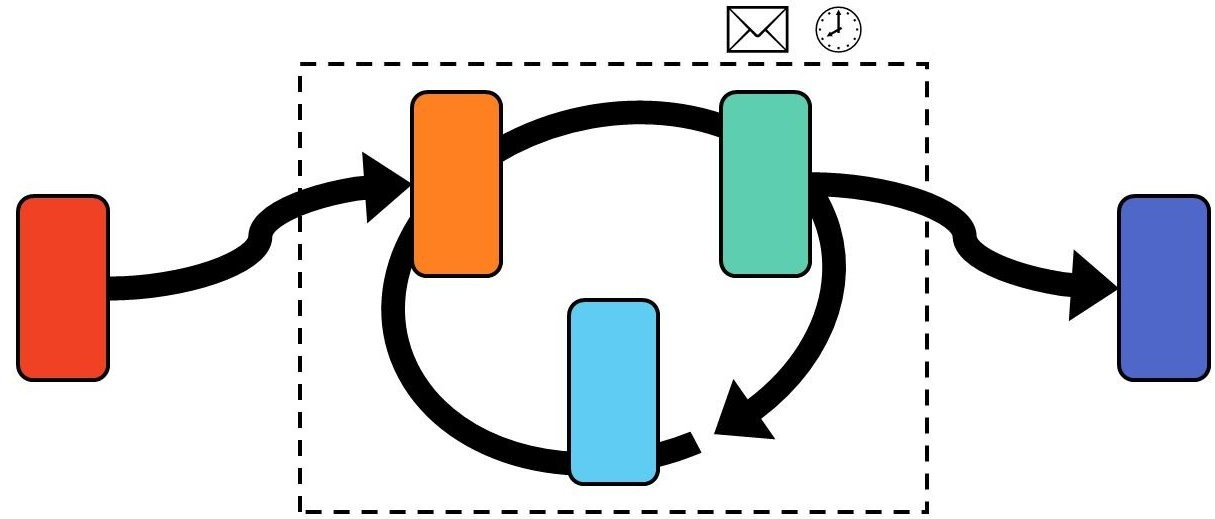
\includegraphics[align=c,width=\linewidth]{img/naiad.jpg}
    Naiad / Timely & 2013~\cite{Naiad2013}
        & 2019~\cite{Timely} & \GreenYes{} & -- \\
    \makecell{
\includegraphics[align=c,width=0.8\linewidth]{img/heron.png} \\ \cite{Heron,kulkarni2015twitter-heron}}
        & 2015 & 2019 & \GreenYes{} & 43 \\
\end{Tabular}

\vspace{1cm}

\caption{A selection of major distributed stream processing systems.}
\label{fig:dsps-examples}
\end{figure}

\section{Ordering and Type Safety}

We introduce and explore using \emph{data-trace types}, previously
discussed in three papers~\citeMain{festschrift18,pldi19,oopsla20},
to solve the problem of encoding ordering requirements in stream processing
systems.
These date back to Mazurkiewicz traces, studied in concurrency theory to model distributed sets of events~\cite{mazurkiewicz1986trace,DiekertR1995}.
These give a kind of semantics to stream processing programs (what it means for
them to be correct) in the presence of out-of-order data.
We also aim to answer the question: what are these types good for?
We explore their use as a programming discipline~\citeMain{pldi19},
implemented on top of Apache Storm~\cite{Storm},
as well as a lightweight testing technique~\citeMain{oopsla20},
implemented on top of Apache Flink~\cite{Flink}.

\subsection{Types for Data Streams}

A \defn{data type} $A = (\Sigma,(T_\sigma)_{\sigma \in \Sigma})$ consists of a potentially infinite \emph{tag alphabet} $\Sigma$ and a value type $T_\sigma$ for every tag $\sigma \in \Sigma$. The set of \emph{elements} of type $A$, or \defn{data items}, is equal to $\{ (\sigma,d) \mid \text{$\sigma \in \Sigma$ and $d \in T_\sigma$} \}$, which we will also denote by $A$. The set of \emph{sequences} over $A$ is denoted as $A^*$. A \defn{dependence relation} on a tag alphabet $\Sigma$ is a symmetric binary relation on $\Sigma$. We say that the tags $\sigma$, $\tau$ are \emph{independent} (w.r.t.\ a dependence relation $D$) if $(\sigma,\tau) \notin D$. For a data type $A = (\Sigma,(T_\sigma)_{\sigma \in \Sigma})$ and a dependence relation $D$ on $\Sigma$, we define the dependence relation that is induced on $A$ by $D$ as
$\{
   ((\sigma,d),(\sigma',d')) \in A \times A \mid
   (\sigma,\sigma') \in D
 \}
$,
which we will also denote by $D$. Define $\eq_D$ to be the smallest congruence (w.r.t.\ sequence concatenation) on $A^*$ containing $\{ (ab,ba) \in A^* \times A^* \mid (a,b) \notin D \}$. Informally, two sequences are equivalent w.r.t.\ $\eq_D$ if one can be obtained from the other by repeatedly commuting adjacent items with independent tags.

\begin{example}
\label{ex:dependence}
Suppose we want to process a stream that consists of sensor measurements and special symbols that indicate the end of a one-second interval. The data type for this input stream involves the tags $\Sigma = \{ \tg M, \tg\# \}$, where $\tg M$ indicates a sensor measurement and $\tg\#$ is an end-of-second marker. The value sets for these tags are $T_{\tg M} = \Nat$ (the natural numbers), and $T_{\tg\#} = \Ut$ is the unit type (singleton). So, the data type $A = (\Sigma,T_{\tg M},T_{\tg\#})$ contains measurements $(\tg M, d)$, where $d$ is a natural number, and the end-of-second symbol $\tg\#$.

The dependence relation $D = \{ (\tg M, \tg\#), (\tg\#, \tg M), (\tg\#,\tg\#) \}$ says that the tag $\tg M$ is independent of itself, and therefore consecutive $\tg M$-tagged items are considered unordered. For example, $(\tg M, 5) \; (\tg M, 5) \; (\tg M, 8) \; \tg\# \; (\tg M, 9)$ and $(\tg M, 8) \; (\tg M, 5) \; (\tg M, 5) \; \tg\# \; (\tg M, 9)$ are equivalent w.r.t.\ $\eq_D$.
\end{example}

A \defn{data-trace type} is a pair $X = (A,D)$, where $A$ is a data type and $D$ is a dependence relation on the tag alphabet of $A$. A \defn{data trace} of type $X$ is a congruence class of the relation $\eq_D$. We also write $X$ to denote the set of data traces of type $X$. Since the equivalence $\eq_D$ is a congruence w.r.t.\ sequence concatenation, the operation of concatenation is also well-defined on data traces: $[u] \cdot [v] = [uv]$ for sequences $u$ and $v$, where $[u]$ is the congruence class of $u$. We define the relation $\leq$ on the data traces of $X$ as a generalization of the prefix partial order on sequences: for data traces $\trc u$ and $\trc v$ of type $X$, $\trc u \leq \trc v$ iff there are $u \in \trc u$ and $v \in \trc v$ s.t.\ $u \leq v$ (i.e., $u$ is a prefix of $v$). The relation $\leq$ on data traces of a fixed type is a partial order. Since it generalizes the prefix order on sequences (when the congruence classes of $\eq_D$ are singleton sets), we will call $\leq$ the \emph{prefix order} on data traces.

\begin{example}[Data Traces]
\label{ex:data-trace}
Consider the data-trace type $X = (A,D)$, where $A$ and $D$ are given in Example~\ref{ex:dependence}. A data trace of $X$ can be represented as a sequence of multisets (bags) of natural numbers and visualized as a partial order on that multiset. The trace corresponding to the sequence of data items
$
  (\tg M, 5) \; (\tg M, 7) \; \tg\# \; (\tg M, 9) \; (\tg M, 8) \; (\tg M, 9) \; \tg\# \; (\tg M, 6)
$
is visualized as:
\newline
\centerline{\small
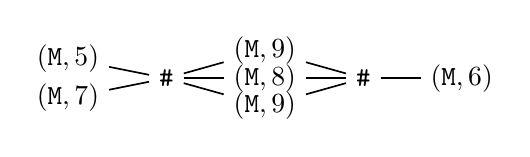
\begin{tikzpicture}[-, >=to, auto, node distance=1.25cm, semithick, transform shape]
\node (M1) {};
\node (T1) [above of=M1, node distance=0.25cm] {$(\tg M,5)$};
\node (B1) [below of=M1, node distance=0.25cm] {$(\tg M,7)$};
\node (M2) [right of=M1] {$\tg\#$};
\node (M3) [right of=M2] {$(\tg M,8)$};
\node (T3) [above of=M3, node distance=0.35cm] {$(\tg M,9)$};
\node (B3) [below of=M3, node distance=0.35cm] {$(\tg M,9)$};
\node (M4) [right of=M3] {$\tg\#$};
\node (M5) [right of=M4] {$(\tg M,6)$};
%
\path (T1) edge (M2);
\path (B1) edge (M2);
\path (M2) edge (T3);
\path (M2) edge (M3);
\path (M2) edge (B3);
\path (T3) edge (M4);
\path (M3) edge (M4);
\path (B3) edge (M4);
\path (M4) edge (M5);
\end{tikzpicture}
}%
\vspace{-1ex}
\newline
where a line from left to right indicates that the item on the right must occur after the item on the left. The end-of-second markers $\tg\#$ separate multisets of natural numbers. So, the set of data traces of $X$ has an isomorphic representation as the set $\Bag(\Nat)^+$ of nonempty sequences of multisets of natural numbers. In particular, the empty sequence $\epsilon$ is represented as $\emptyset$ and the single-element sequence $\tg\#$ is represented as $\emptyset \; \emptyset$.
\end{example}

A singleton tag alphabet can be used to model sequences or multisets over a basic type of values. For the data type given by $\Sigma = \{\sigma\}$ and $T_\sigma = T$ there are two possible dependence relations for $\Sigma$, namely $\emptyset$ and $\{(\sigma,\sigma)\}$. The data traces of $(\Sigma,T,\emptyset)$ are multisets over $T$, which we denote as $\Bag(T)$, and the data traces of $(\Sigma,T,\{(\sigma,\sigma)\})$ are sequences over $T$.

\begin{example}[Multiple Input/Output Channels]
\label{ex:channels}
Suppose we want to model a streaming system with multiple independent input and output channels, where the items within each channel are linearly ordered but the channels are completely independent. This is the setting of (acyclic) \emph{Kahn Process Networks} ~\cite{gilles1974semantics} and the more restricted synchronous dataflow models \cite{lee1987synchronous, benveniste2003synchronous}. We introduce tags $\Sigma_\tg{I} = \{ \tg{I}_1, \ldots, \tg{I}_m \}$ for $m$ input channels, and tags $\Sigma_\tg{O} = \{ \tg{O}_1, \ldots, \tg{O}_n \}$ for $n$ output channels.
The dependence relation for the input consists of all pairs $(\tg{I}_i,\tg{I}_i)$ with $i = 1, \ldots, m$. This means that for all indexes $i \neq j$ the tags $\tg{I}_i$ and $\tg{I}_j$ are independent. Similarly, the dependence relation for the output consists of all pairs $(\tg{O}_i,\tg{O}_i)$ with $i = 1, \ldots, n$. Assume that the value types associated with the input tags are $T_1$, \ldots, $T_m$, and the value types associated with the output tags are $U_1$, \ldots, $U_n$. The sets of input and output data traces are (up to a bijection) $T^*_1 \times \cdots \times T^*_m$ and $U^*_1 \times \cdots \times U^*_m$ respectively.
\end{example}

\subsection{Type-Consistent Programming}

Data-trace types are useful for giving the meaning (semantics) of a stream processing system. Consider the analogy with a functional model of computation: the meaning of a program consists of the input type, the output type, and a mapping that describes the input/output behavior of the program. Correspondingly, the semantics for a stream processing systems consists of:
\begin{enumerate}
\item
the type $X$ of input data traces,
\item
the type $Y$ of output data traces, and 
\item
a monotone mapping $\beta: X \to Y$ that specifies the cumulative output after having consumed a prefix of the input stream.
\end{enumerate}
The monotonicity requirement captures the idea that output items cannot be retracted after they have been omitted. Since $\beta$ takes an entire input history (data trace) as input, it can model stateful systems, where the output that is emitted at every step depends potentially on the entire input history.

We have already discussed how (monotone) functions from $A^*$ to $B^*$ model sequential stream processors. We will now introduce the formal notion of \emph{consistency}, which captures the intuition that a sequential implementation does not depend on the relative order of any two elements unless the stream type considers them to be relatively ordered.

\begin{definition}[Consistency]
Let $X = (A,D)$ and $Y = (B,E)$ be data-trace types. We say that a data-string transduction $f: A^* \to B^*$
is \emph{$(X,Y)$-consistent} if $u \eq_D v$ implies that $\bar{f}(u) \eq_{E} \bar{f}(v)$ for all $u, v \in A^*$.

Let $f \in A^* \to B^*$ be a $(X,Y)$-consistent data-string transduction. The function $\beta: X \to Y$, defined by
$\beta([u]) = [\bar f(u)]$ for all $u \in A^*$, is called the \emph{$(X,Y)$-denotation} of $f$.
\end{definition}

\begin{definition}[Data-Trace Transductions]
Let $X = (A,D)$ and $Y = (B,E)$ be data-trace types. A \textbf{\em data-trace transduction} with input type $X$ and output type $Y$ is a function $\beta: X \to Y$ that is monotone w.r.t.\ the prefix order on data traces: $\trc u \leq \trc v$ implies that $\beta(\trc u) \leq \beta(\trc v)$ for all traces $\trc u, \trc v \in X$. 
\end{definition}

It is shown in \cite{festschrift18} that the set of data-trace transductions from $X$ to $Y$ is equal to the set of $(X,Y)$-denotations of all $(X,Y)$-consistent data-string transductions.

We define two kinds of \textbf{\em data-trace types} for streams of key-value pairs: \emph{unordered} types of the form $\Unord(K,V)$, and \emph{ordered} types of the form $\Ord(K,V)$. For a set of keys $K$ and a set of values $V$, let $\Unord(K, V)$ denote the type with alphabet $K \cup \{\tg\#\}$, values $V$ for every key, values $\Nat$ for the $\tg\#$ tag (i.e., marker timestamps), and dependence relation $\{ (\tg\#, \tg\#) \} \cup \{ (k,\tg\#), (\tg\#,k) \mid k \in K \}$. In other words, $\Unord(K, V)$ consists of data traces where the marker tags $\tg\#$ are linearly ordered and the elements between two such tags are of the form $(k,v)$, where $k \in K$ and $v \in V$, and are completely unordered. We define $\Ord(K, V)$ similarly, with the difference that the dependence relation also contains $\{ (k,k) \mid k \in K \}$. That is, in a data trace of $\Ord(K,V)$, elements with the same key are linearly ordered between $\tg\#$ markers, but there is no order across elements of different keys.

A \textbf{\em transduction DAG} is a tuple $(S,N,T,E,\to,\lambda)$ which represents a labelled directed acyclic graph, where: $S$ is the set of \emph{source vertices}, $T$ is the set of \emph{sink vertices}, $N$ is the set of \emph{processing vertices}, $E$ is the set of \emph{edges} (i.e., connections/channels), $\to$ is the \emph{edge relation}, and $\lambda$ is a \emph{labelling function}. The function $\lambda$ assigns: (1) a data-trace type to each edge, (2) a data-trace transduction to each processing vertex that respects the input/output types, and (3) names to the source/sink vertices. We require additionally that each source vertex has exactly one outgoing edge, and each sink vertex has exactly one incoming edge.

\begin{example}[Time-Series Interpolation]
\label{ex:IoT}
Consider a home IoT system where temperature sensors are installed at a residence. We wish to analyze the sensor time series to create real-time notifications for excessive energy loss through the windows. The sensor time series sometimes have missing data points, and therefore the application requires a pre-processing step to fill in any missing measurements using linear interpolation. We assume that the sensors first send their measurements to a hub, and then the hub propagates them to the stream processing system. The stream that arrives from the hub does not guarantee that the measurements are sent in linear order (e.g., with respect to a timestamp field). Instead, it produces synchronization markers every 10 seconds with the guarantee that all elements with timestamps $< 10 \cdot i$ have been emitted by the time the $i$-th marker is emitted. That is, the $i$-th marker can be thought of as a watermark with timestamp $10 \cdot i$. The input stream is a data trace of $\Unord(\Ut,\texttt{M})$, where $\texttt{M}$ is the type of measurements $(\mathit{id}, \mathit{value}, \mathit{ts})$ consisting of a sensor identifier $id$, a scalar value $value$, and a timestamp $ts$. This is a transduction DAG that describes the pre-processing computation:
\newline
\centerline{%
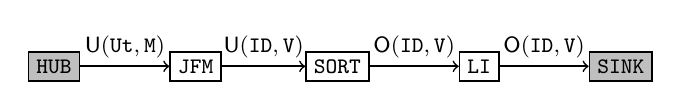
\begin{tikzpicture}[->, >=to, auto, node distance=1.8cm, semithick, transform shape]
%
\footnotesize
%
\node (A) [draw, fill=lightgray] {\texttt{HUB}};
\node (B) [draw, right of=A] {\texttt{JFM}};
\node (C) [draw, right of=B] {\texttt{SORT}};
\node (D) [draw, right of=C] {\texttt{LI}};
\node (E) [draw, fill=lightgray, right of=D] {\texttt{SINK}};
%
\path (A) edge node {$\Unord(\Ut,\texttt{M})$} (B);
\path (B) edge node {$\Unord(\texttt{ID},\texttt{V})$} (C);
\path (C) edge node {$\Ord(\texttt{ID},\texttt{V})$} (D);
\path (D) edge node {$\Ord(\texttt{ID},\texttt{V})$} (E);
%
\end{tikzpicture}
}% end of centerline
\newline
The vertex \texttt{HUB} represents the source of sensor measurements, and the vertex \texttt{SINK} represents the destination of the output stream. \texttt{ID} is the type of sensor identifiers, and \texttt{V} is the type of timestamped values $(\mathit{value}, \mathit{ts})$. The processing vertices are described below:
\begin{itemize}
\item
The stage Join-Filter-Map (\texttt{JFM}) joins the input stream with a table that indicates the location of each sensor, filters out all sensors except for those that are close to windows, and reorganizes the fields of the input tuple.
\item
Recall the guarantee for the synchronization markers, and notice that it implies the following property for the input traces: for any two input measurements that are separated by at least one marker, the one on the left has a strictly smaller timestamp than the one on the right. The sorting stage \texttt{SORT} sorts for each sensor the measurements that are contained between markers.
\item
The linear interpolation stage \texttt{LI} considers each sensor independently and fills in any missing data points.
\end{itemize}
We have described informally the data-trace transductions \texttt{JFM}, \texttt{SORT} and \texttt{LI}. The transduction DAG shown earlier denotes a data-trace transduction $\Unord(\Ut,\texttt{M}) \to \Ord(\texttt{ID},\texttt{V})$.
\end{example}

The computation performed by a processing node is given in a structured fashion, by completing function definitions of a specified \textbf{\em operator template}. Table~\ref{table:templates} shows the three templates that are supported, which encompass both ordered and unordered input streams. Each operator is defined by a sequential implementation, which we describe informally below. This means that each operator can be modeled as a data-string transduction. It can then be proved formally that these data-string transductions are consistent w.r.t.\ their input/output data-trace types. It follows that each operator that is programmed according to the template conventions has a denotation (semantics) as a data-trace transduction of the appropriate type.

\texttt{\bfseries OpStateless}:
The simplest template concerns \emph{stateless} computations, where only the current input event---not the input history---determines the output. The programmer fills in two function definitions: (1) \texttt{onItem} for processing key-value pairs, and (2) \text{onMarker} for processing synchronization markers. The functions have no output (the output type is \texttt{Ut}, i.e.\ the unit type) and their only side-effect is emitting output key-value pairs to the output channel by invoking $\texttt{emit(outputKey, outputValue)}$.

\texttt{\bfseries OpKeyedOrdered}:
Assuming that the input is ordered per key, this template describes a stateful computation for each key independently that is order-dependent. The programmer fills in three function definitions: (1) \texttt{initialState} for obtaining the initial state, (2) \texttt{onItem} for processing a key-value pair and updating the state, and (3) \texttt{onMarker} for processing a synchronization marker and updating the state. The functions have output $S$, which is the type of the data structure for representing the state. As for stateless computations, the functions allow the side-effect of emitting output key-value pairs to the output channel. This template requires a crucial \emph{restriction} for maintaining the order for the output: every occurrence of \texttt{emit} must preserve the input key. If this restriction is violated, e.g.\ by projecting out the key, then the output cannot be viewed as being ordered.

\texttt{\bfseries OpKeyedUnordered}:
Assuming that the input is unordered, this template describes a stateful computation for each key independently. Recall that the synchronization markers are ordered, but the key-value pairs between markers are \emph{unordered}. To guarantee that the computation does not depend on some arbitrary linear ordering of the key-value pairs, their processing does not update the state. Instead, the key-value pairs between two consecutive markers are aggregated using the operation of a \emph{commutative monoid} $A$: the programmer specifies an identity element $\texttt{id()}$, and a binary operation $\texttt{combine()}$ that must be \emph{associative} and \emph{commutative}. Whenever the next synchronization marker is seen, \texttt{updateState} is used to incorporate the aggregate (of type $A$) into the state (of type $S$) and then \texttt{onMarker} is invoked to (potentially) emit output. The behavior \texttt{onItem} may depend on the last snapshot of the state, i.e.\ the one that was formed at the last marker. The functions \texttt{onItem} and \texttt{onMarker} are allowed to emit output data items (but not markers), but the rest of the functions must be pure (i.e., no side-effects).

\begin{theorem}
\normalfont
Every streaming computation defined using the operator templates above is consistent w.r.t.\ its input/output type.
\end{theorem}


\subsection{Runtime Testing}

In this section we describe how the programmer writes specifications in DiffStream~\citeMain{oopsla20}.
Let's look back at the taxi example from before. The second stage of the program
computes the total distance traveled by each taxi by computing the
distance between the current and the previous location, and adding
that to a sum. For this computation to return correct results,
location events for each taxi should arrive in order in its input---a
requirement that must be checked if we want to test the first stage of
the program. We propose expressing this ordering requirement using a
\emph{dependence relation} $D$. The concept of dependence relations
was first introduced in research on concurrency theory, where it was
used to define Mazurkiewicz traces, i.e. partially ordered sequences
of events in distributed systems~\cite{mazurkiewicz1986trace},
and has previously been used to give semantics for stream processing programs~\cite{mamouras2019data}.

A dependence relation is a symmetric binary relation on events of a
stream with the following semantics.
If $x \dep y$, then the order of
$x$ and $y$ in a stream is significant and reordering them gives us
two streams that are not equivalent. This could be the case if the
consumer of an output stream produces different results depending on
the order of $x$ and $y$.  Thus, the dependence relation can be
thought of as encoding the pairwise ordering requirements of the
downstream consumer.

\begin{figure}[t]
  \centering \footnotesize{}
  \begin{subfigure}[b]{0.46\textwidth}
    \centering
    \begin{lstlisting}[basicstyle=\ttfamily\small]
  (ev1, ev2) ->
      ev1.taxiID == ev2.taxiID
    \end{lstlisting}
    \caption{Specification in DiffStream}
    \label{fig:simple-taxi-example-dependency-spec}
  \end{subfigure}%
  \qquad
  \begin{subfigure}[b]{0.46\textwidth}
    \centering
    \KeyDepGraph{tID}
    \caption{Dependence visualized as a graph}
    \label{fig:simple-taxi-example-dependency-vis}
  \end{subfigure}%
  \caption{Example specification in DiffStream for the taxi example. Taxi events with the same \inljava{taxiID} are dependent.}
  \label{fig:example-dependencies}
\end{figure}

It is often helpful to visualize dependence relations as unordered
graphs, where nodes are equivalence classes of the dependence
relation. For the taxi example, the dependence relation is visualized
in Figure~\ref{fig:simple-taxi-example-dependency-vis}, and it indicates that
events with the same taxi identifier are dependent. In DiffStream,
dependence relations can be specified using a Boolean function on a pair
of events. These functions should be pure and should only depend on
the fields of the two events. The DiffStream specification of the dependence relation from Figure~\ref{fig:simple-taxi-example-dependency-vis} is shown in Figure~\ref{fig:simple-taxi-example-dependency-spec}.

\begin{figure}[t]
  \centering \footnotesize{}
  \begin{subfigure}[b]{0.56\textwidth}
    \centering
    \begin{lstlisting}[basicstyle=\ttfamily\small,linewidth=7.3cm]
  (ev1, ev2) ->
      ev1.isEOD() ||
      ev2.isEOD() ||
      (ev1.isEOM() && ev2.isEOM()) ||
      (ev1.isTaxiEv() &&
       ev2.isTaxiEv() &&
       ev1.taxiID == ev2.taxiID)
    \end{lstlisting}
    \caption{Specification in DiffStream}
    \label{fig:extended-taxi-example-dependency-spec}
  \end{subfigure}%
  \qquad
  \begin{subfigure}[b]{0.36\textwidth}
    \centering
    \ExtendedKeyDepGraph{tID}
    \caption{Dependence visualized as a graph}
    \label{fig:extended-taxi-example-dependency-vis}
  \end{subfigure}
  \caption{Example specification in DiffStream for the extended taxi example. Taxi events with the same \inljava{taxiID} are dependent
      and all events are dependent with end-of-day (EOD) events.}
  \label{fig:extended-example-dependencies}
\end{figure}

Now let's consider an extension of the above example where the downstream consumer
computes the total distance traveled by each taxi \emph{per
  day}, and also computes the average daily distance by each taxi
every month. To make this possible, the output of the program under test
is now
extended with special EOD (\emph{end-of-day}) and EOM (\emph{end-of-month})
events. The ordering requirements on this output, while more subtle, can still be
precisely specified using a dependence relation.
For example, EOD events are dependent with taxi events since all events of a specific day have to occur before the EOD event of that day for the total daily distance to be correctly computed. On the other hand, EOM events do not have to be dependent with taxi events since daily distances are computed on EOD events. Therefore, an EOM event can occur anywhere between the last EOD event of the month and the first EOD event of the next month.
The DiffStream specification of the dependence relation and its visualization are both shown in Figure~\ref{fig:extended-example-dependencies}.

\begin{figure}[t]
  \centering \footnotesize{}
\begin{tabular}{c}
\begin{lstlisting}[basicstyle=\ttfamily\small,linewidth=9cm]
  (ev1, ev2) -> distance(ev1.loc, ev2.loc) < 1
\end{lstlisting}
\end{tabular}
  \caption{Example specification in DiffStream where  events are dependent if their locations are close.}
  \label{fig:proximity-example-dependencies}
\end{figure}

Several frequently occurring dependence relations can be specified
using a combination of the predicates seen in the above examples. This
includes predicates that check if an event is of a specific type
(e.g. \inljava{isEOD()}, \inljava{isTaxiEv()}), and predicates that
check a field (possibly denoting a key or identifier) of the two
events for equality (e.g. \inljava{ev1.taxiID ==
  ev2.taxiID}). However, it is conceivable that the dependence of two
events is determined based on a complex predicate on their fields.

\begin{figure}[t]
  \centering \footnotesize{}
\begin{tabular}{c}
\begin{lstlisting}[basicstyle=\ttfamily\small,linewidth=10cm]
  (ev1, ev2) -> (ev1.isPunctuation() &&
                 ev2.timestamp < ev1.timestamp) ||
                (ev2.isPunctuation() &&
                 ev1.timestamp < ev2.timestamp)
\end{lstlisting}
\end{tabular}
  \caption{Example specification in DiffStream where punctuation events, used to enforce progress, depend on other events only if the punctuation timestamp is larger.}
  \label{fig:punctuation-example-dependencies}
\end{figure}

Another interesting dependence relation occurs in cases where output streams contain punctuation events.
Punctuations are periodic events that contain a timestamp and indicate
that all events up to that timestamp, i.e. all events \inljava{ev} such that \inljava{ev.timestamp < punc.timestamp}, have \emph{most likely} already occurred.
Punctuation events allow programs to make progress, completing any
computation that was waiting for events with earlier
timestamps. However, since events could be arbitrarily delayed, some
of them could arrive after the punctuation.
Consider as an example a taxi that briefly
disconnects from the network and sends the events produced while disconnected
after it reconnects with the network. These events are usually
processed with a custom out-of-order handler, or are completely
dropped. Therefore, punctuation events are dependent with events
that have an earlier timestamp, since reordering them alters the result of the computation, while they are independent of events with later timestamps. This can be specified in DiffStream as
shown in Figure~\ref{fig:punctuation-example-dependencies}.

\begin{algorithm}[t]
  \renewcommand{\thealgorithm}{DiffStream}
  \caption{Checking equivalence of two streams}
  \label{alg:equivalence}
  \begin{algorithmic}[1]
    \Require Equality relation $\equiv$, dependence relation $\dep$
    \Require Connected stream $s$ with $\pi_1(s)=s_1$ and $\pi_2(s)=s_2$
    \renewcommand{\algorithmicrequire}{\textbf{Require:}}
    \Require Relations $\equiv$ and $\dep$ are compatible
    \Function{StreamsEquivalent}{$s$}
    \label{line:StreamsEquivalentBegin}
    \State $u_1, u_2 \gets$ empty logically ordered sets
    \State {\color{gray}Ghost state: $p_1, p_2 \gets$ empty logically ordered sets}
    \State {\color{gray}Ghost state: $f \gets$ empty function $p_1\to p_2$}
    \For{$(x, i)$ in $s$}\label{line:ProcessElementBegin}
      \State $j \gets 3-i$
      \If{$x$ is minimal in $u_i$ and $\exists y\in \min u_j: x \equiv y$}
      \label{line:MatchBegin}
        \State $u_j \gets u_j \setminus \{y\}$
        \State {\color{gray}$p_i \gets p_i \cup \{x\}$};
        {\color{gray}$p_j \gets p_j \cup \{y\}$}\label{line:GhostBegin}
        \State {\color{gray}$f \gets f[x\mapsto y]$ \textbf{if} $i=1$
          \textbf{else} $f[y\mapsto x]$}\label{line:MatchEnd}
      \ElsIf{$\exists y \in u_j: x \dep y$}\label{line:NotEquivalentBegin}
        \State \textbf{return false}\label{line:NotEquivalentEnd}
      \Else\label{line:UnmatchedBegin}
        \State $u_i \gets u_i \cup \{x\}$\label{line:UnmatchedEnd}
      \EndIf\label{line:ProcessElementEnd}
    \EndFor
    \State \textbf{return} ($u_1=\emptyset$ and $u_2=\emptyset$)
    \label{line:FiniteEquivalent}
    \EndFunction\label{line:StreamsEquivalentEnd}
  \end{algorithmic}
\end{algorithm}

\begin{figure}[tb]
    \centering \small
\begin{tabular}{c}
\begin{lstlisting}[linewidth=9.5cm]
public void testKeyBy() throws Exception {
    StreamExecutionEnvironment env = ...;

    DataStream input = generateInput(env);

    StreamEquivalenceMatcher matcher =
        StreamEquivalenceMatcher.createMatcher(
            sequentialImpl(input), parallelImpl(input),
            (ev1, ev2) -> ev1.taxiID == ev2.taxiID);

    env.execute();
    matcher.assertStreamsAreEquivalent();
}
\end{lstlisting}
\end{tabular}
    \caption{An example test in DiffStream.}
    \label{fig:keybytest}
\end{figure}{}

\begin{figure}[tb]
    \centering \small

    \setlength\tabcolsep{1em}
    \begin{tabular}{c|ccc}
          & \multicolumn{3}{c}{\underline{Application-Specific Requirements}} \\
         Code pattern & Determinism & \makecell{Determinism under \\ input assumptions} & \makecell{None \\ (nondeterminism acceptable)} \\
         \hline
         \texttt{SingleItem} & \cmark{} & \cmark{} & n/a \\
         \texttt{IndexValuePair} & \cmark{} & \cmark{} & n/a \\
         \texttt{MaxRow} & \cmark{} & \cmark{} & \xmark{} \\
         \texttt{FirstN} & \cmark{} & \cmark{} & \xmark{} \\
         \texttt{StrConcat} & \cmark{} & n/a & \cmark{} \\
    \end{tabular}

    \caption{Results of the MapReduce case study. A \cmark{} indicates successfully identifying the bug in the first column, and successfully avoiding a false positive in the second and third columns, for each of the 5 reducers implemented.}
    \label{fig:mapreduce-case-study-summary}
\end{figure}

\begin{figure}[t!]
    \centering
    \begin{subfigure}[t]{0.33\textwidth}
        \centering
        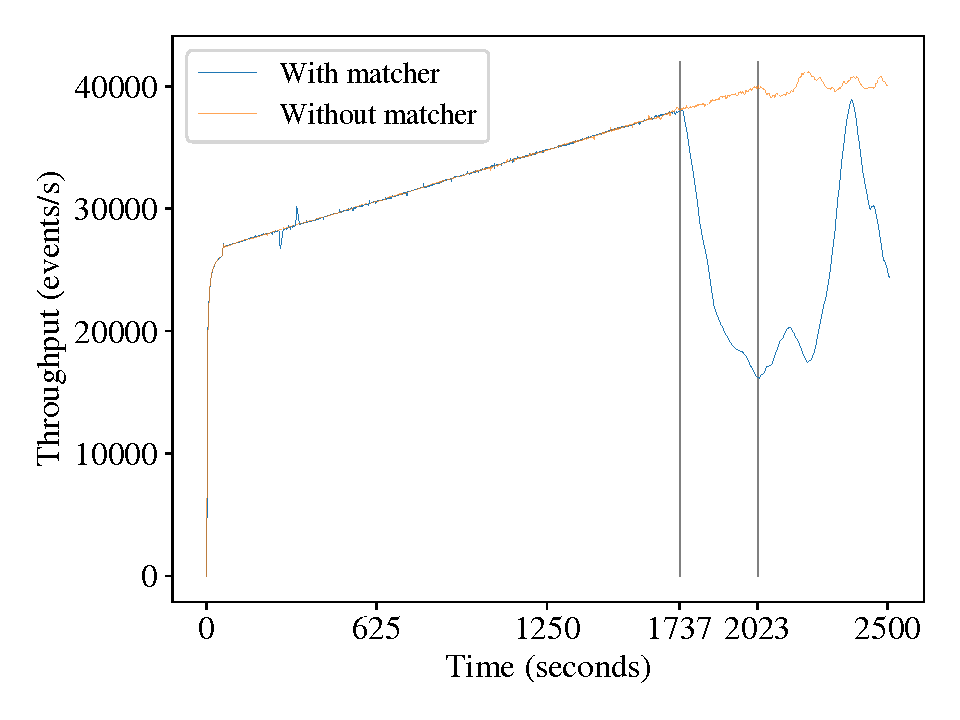
\includegraphics[width=1.0\textwidth]{figures/diffstream/throughput-accelerated.pdf}
        \caption{}\label{fig:throughput}
    \end{subfigure}%
    \begin{subfigure}[t]{0.33\textwidth}
        \centering
        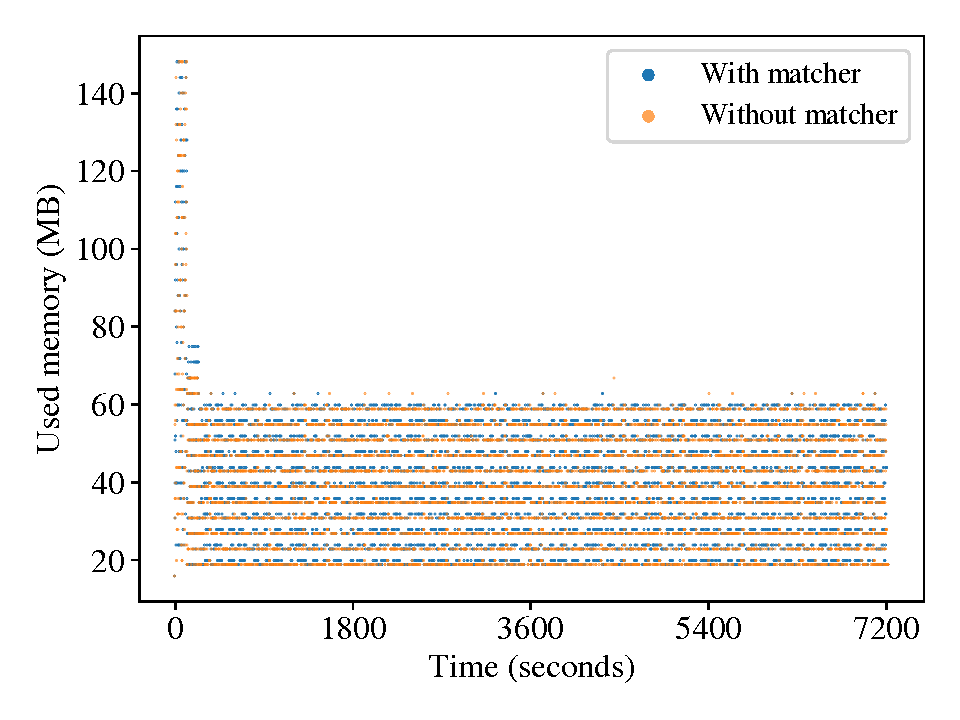
\includegraphics[width=1.0\textwidth]{figures/diffstream/used_memory_in_time.pdf}
        \caption{}\label{fig:memory-in-time}
    \end{subfigure}%
    \begin{subfigure}[t]{0.33\textwidth}
        \centering
        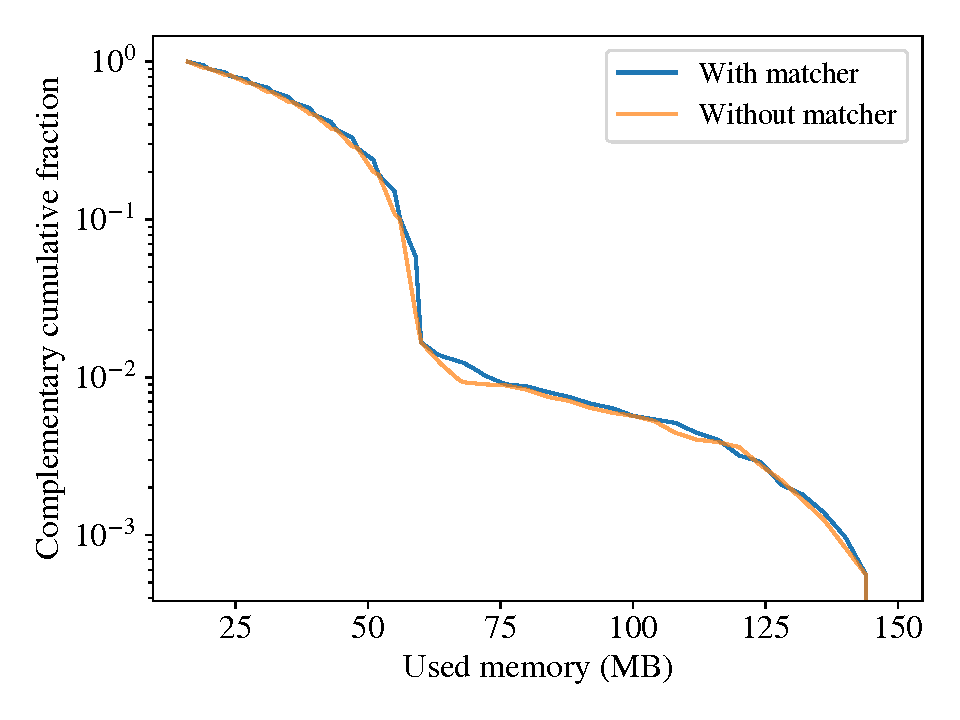
\includegraphics[width=1.0\textwidth]{figures/diffstream/memory_ccdf.pdf}
        \caption{}\label{fig:memory-ccdf}
    \end{subfigure}%
    \\
    \begin{subfigure}[t]{0.33\textwidth}
        \centering
        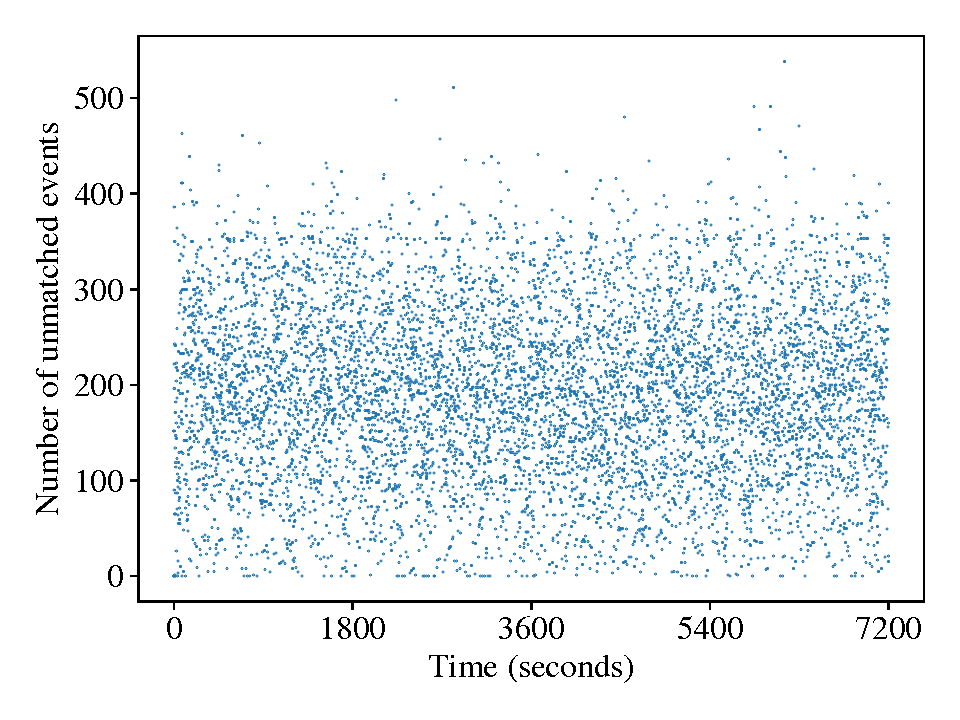
\includegraphics[width=1.0\textwidth]{figures/diffstream/unmatched_in_time.pdf}
        \caption{}\label{fig:unmatched-in-time}
    \end{subfigure}%
    \begin{subfigure}[t]{0.33\textwidth}
        \centering
        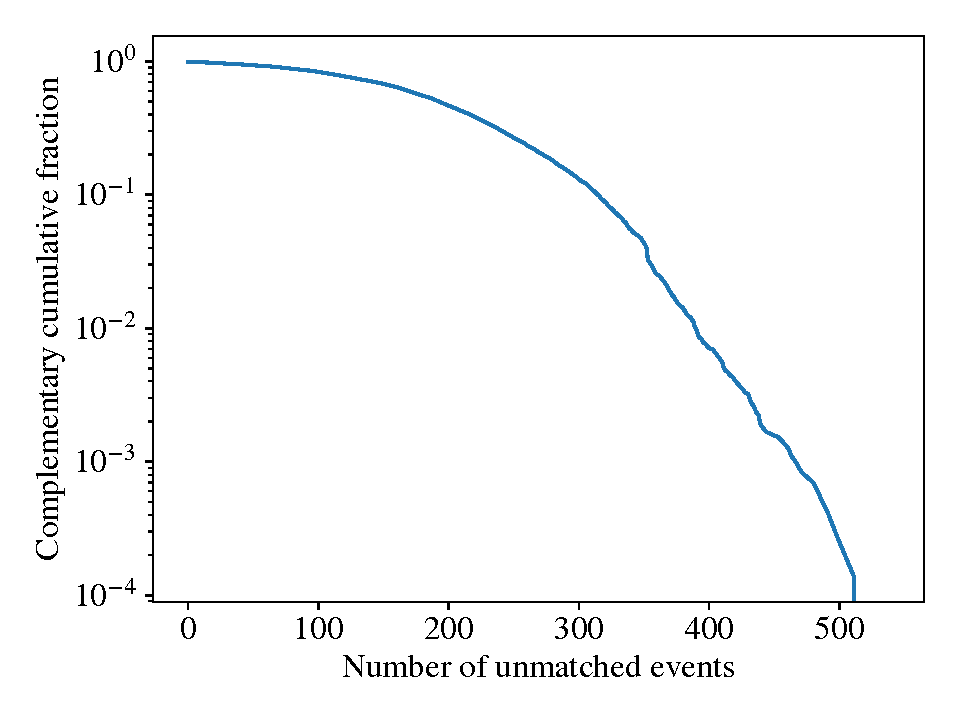
\includegraphics[width=1.0\textwidth]{figures/diffstream/unmatched_ccdf.pdf}
        \caption{}\label{fig:unmatched-ccdf}
    \end{subfigure}%
    \begin{subfigure}[t]{0.33\textwidth}
        \centering
        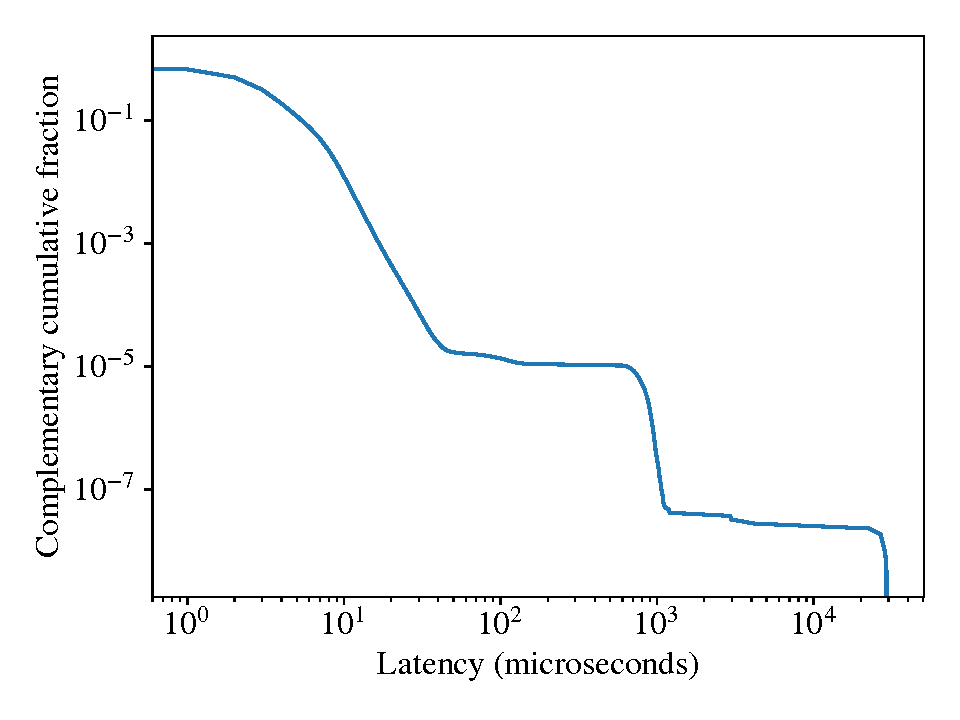
\includegraphics[width=1.0\textwidth]{figures/diffstream/latencies.pdf}
        \caption{}\label{fig:latencies}
    \end{subfigure}
    \caption{Results of the fourth case study: performance measurements of monitoring an application with DiffStream on the Yahoo streaming benchmark over a span of 2 hours, compared to the same application without the DiffStream matcher.}
\label{fig:online-perf-results}
\end{figure}

\subsection{Discussion and Directions}

\section{Execution Models}

\citeMain{icalp17,popl19,tcs20}

\subsection{Data Transducers}

To model data streams we use \emph{data words}.
Let $\data$ be a (possibly infinite) set of \defn{data values},
such as the set of integers or real numbers,
and let $\Sigma$ be a finite set of \defn{tags}.
Then a \defn{data word} is a sequence of tagged data values
$\dw{w} \in (\Sigma \times \data)^*$.
We write $\dw{w} \downarrow \Sigma$ to denote
the projection of $\dw{w}$ to a string in $\Sigma^*$.
We use bold $\dw{u}$, $\dw{v}$, $\dw{w}$ to denote data words.
We reserve non-bold $u, v, w$ for plain strings of tags in $\Sigma^*$.
We write $d, d_i$ for elements of $\data$.
We use $\sigma$ to denote an arbitrary tag in $\Sigma$,
and in the examples we write particular tags in typewriter font, e.g. $\tg{a}, \tg{b}$.

A \defn{signature} is a tuple $(\data, \ops)$,
where $\data$ is a set of data values
and $\ops$ is a set of \defn{allowed operations}.
Each operation has an \defn{arity} $k \ge 0$
and is a function from $\data^k$ to $\data$.
We use $\ops_k$ to denote the $k$-ary operations.
For instance, if $\data$ is all 64-bit integers, we might support 64-bit arithmetic, as well as
integer division and equality tests.
Alternatively we might have $\data = \mathbb{N}$
with the operations $+$ (arity 2), $\min$ (arity 2), and $0$ (arity 0).
In general, we may have arbitrary user-defined operations on $\data$.
Given a signature $(\data, \ops)$,
and a collection of variables $Z$,
the set of \defn{terms} $\tms[Z]$
consists of all syntactically correct expressions
with free variables in $Z$, using operations $\ops$.
So $\min(x,0) + \min(y,0)$ and $x + x$
are terms over the signature $(\mathbb{N}, \{+,\min,0\})$ with $Z = \{x,y\}$.

We define two special values in addition to
the values in $\data$: $\bot$ denotes \defn{undefined}
and $\top$ denotes \defn{conflict}.
We let $\cdata := \data \cup \{\bot, \top\}$ be the set of \defn{extended data values},
and refer to elements of $\data$ as \defn{defined}.
We lift $\ops$ to operations on $\cdata$ by thinking of $\bot$ as the empty multiset,
elements of $\data$ as singleton multisets, and $\top$ as any multiset of two or more data values.
The specific behavior of $\op \in \ops$ on values in $\cdata$
is illustrated in the table below
for the case $\op \in \ops{}_2$.
We also define a \defn{union} operation $\sqcup: \cdata \times \cdata \to \cdata$:
if either of its arguments is undefined it returns the other one,
and in all other cases it returns conflict.
This represents multiset union. Note that $d_1 \sqcup d_2 = \top$ even if $d_1 = d_2$.
This is essential: it guarantees that for all operations on extended data values, whether the result is undefined, defined, or conflict can be determined from knowing only whether the inputs are undefined, defined, or conflict.
(For instance, we rely on this guarantee for the theorems in \S\ref{subsec:dt-regularity} and for the translation from QRE-Past in \S\ref{subsec:rm-compilation}. It's not needed for most of the constructions in \S\ref{sec:constructions}.)
\[
\small
\begin{array}{c|ccc}
\sqcup & \bot & d_2 & \top \\
\hline
\bot & \bot & d_2 & \top \\
d_1 & d_1 & \top & \top \\
\top & \top & \top & \top
\end{array}
\qquad \qquad
\begin{array}{c|ccc}
\op & \bot & d_2 & \top \\
\hline
\bot & \bot & \bot & \bot \\
d_1 & \bot & \hspace{-5pt}\op(d_1,d_2)\hspace{-5pt} & \top \\
\top & \bot & \top & \top
\end{array}
\]

$\cdata$ is a \emph{complete lattice}, partially ordered under the
relation $\le$ which is defined by $\bot \le d \le \top$ for all $d \in \data$,
and distinct elements $d, d' \in \data$ are incomparable.
For a finite set $X$, we write the set of functions $X \to \cdata$ as $\cdata^X$; its elements are un-tagged \defn{data vectors}, denoted $\dv{x}$, $\dv{y}$.
The partial order extends coordinate-wise to an ordering $\dv{x} \le \dv{y}$ on data vectors $\dv{x}, \dv{y} \in \cdata^X$.
All operations in $\ops{}$ are \emph{monotone increasing}
w.r.t. this partial order.
Union ($\sqcup$) is commutative and associative, with identity $\bot$ and absorbing element $\top$,
and \emph{all} $k$-ary operations distribute over it.

%%%%%%%%%%%%%%%%%%%%%%%%%%%%%%%%%%%%%%%%%%%%%%%%%%%

\paragraph*{Syntax.}
Let $(\data, \ops)$ be a fixed signature.
A \defn{data transducer (DT)} is a 5-tuple $\DT = \DTtuple$, where:
\begin{itemize}
\item $\states$ is a finite set of \defn{state variables} (\defn{states} for short) and $\tags$ is a finite set of \defn{tags}.
We write $\states'$ for a copy of the variables in $\states$: for $q \in \states$, $q' \in \states'$ denotes the copy. When the states of the DT are updated, $q'$ will be the new, updated value of $q$.
\item $\update$ is a finite set of \defn{transitions},
where each transition is a tuple $(\sigma, X, q', t)$.
\begin{itemize}
\item $\sigma \in \Sigma \cup \{\tg{i}\}$,
where $\tg{i} \notin \Sigma$, and if $\sigma = \tg{i}$ this is a special \emph{initial transition}.
\item $X \subseteq \states \cup \states'$ is a set of
\emph{source variables} and $q' \in \states'$ is the \emph{target variable}.
\item $t \in \tms[X \cup \{\curritem\}]$ gives a new value of the target variable given values of the source variables
and given the value of ``$\curritem$'', which represents the current data value in the input data word.
Assume that $\curritem \notin X$.
We allow $X$ to include some variables not used in $t$.
For initial transitions, we additionally require that $X \subseteq \states'$ and that $\curritem$ does not appear in $t$.
\end{itemize}
\item $\init \subseteq \states$ is a set of \emph{initial states} and $\final \subseteq \states$ is a set of \emph{final states}.
\end{itemize}

The \defn{number of states} of $\DT$ is $|\states|$.
The \defn{size} of $\DT$ is the the number of states plus the total length of all transitions
$(\sigma, X, q', t)$, which includes the length of description of all the terms $t$.

\paragraph*{Semantics.}
The input to a DT has two components.
First, an \defn{initial vector} $\dv{x} \in \cdata^\init$, which assigns an extended data value to each initial state. Second, an \defn{input data word} $\dw{w} \in (\Sigma \times D)^*$, which is a sequence of tagged data values to be processed by the transducer. On input $(\dv{x},\dw{w})$, the DT's final \defn{output vector} is an extended data value at each of its final states.
Thus, the semantics of $\DT$ will be
\[
\sem{\DT} : \cdata^\init \times (\tags \times \data)^* \to \cdata^\final.
\]

A \defn{configuration} is a vector $\dv{c} \in \cdata^\states$.
For every $\sigma \in \Sigma$, the set of transitions $(\sigma, X, q', t)$
collectively define a function $\update_\sigma : \cdata^\states \times \data \to \cdata^\states$:
given the current configuration and the current data value from the input data word,
$\update_\sigma$ produces the next configuration.
We define $\update_\sigma(\dv{c},d)(q) := \dv{c}'(q')$,
where $\dv{c}' \in \cdata^{Q \cup Q' \cup \{\curritem\}}$ is the \emph{least vector} satisfying
$\dv{c}'(\curritem) = d$; for all $q \in Q$, $\dv{c}'(q) = \dv{c}(q)$;
and
\begin{equation}
\text{for all }q' \in Q',\quad
\dv{c}'(q') = \bigsqcup_{(\sigma, X, q', t) \in \update} \sem{t}(\dv{c}'|_X),
\label{eq:fixpoint-semantics}
\end{equation}
where we define $\sem{t}(\dv{c}'|_X)$ to be $\bot$ if there exists $x \in X$ such that $\dv{c}'(x) = \bot$; otherwise, $\top$ if there exists $x \in X$ such that $\dv{c}'(x) = \top$; otherwise, if all variables in $X$ are defined, then $\sem{t}(\dv{c}'|_X)$ is the value of the expression $t$ with variables assigned the values in $\dv{c}'$.
So, $\sem{t}(\dv{c}'|_X)$ produces $\bot$ or $\top$ if some variable in $X$ is $\bot$ or $\top$.
The above union is over all transitions with label $\sigma$ and target variable $q'$.
Since $\cdata$ is a complete lattice, this least fixed point exists by the Knaster-Tarski theorem.

The case of initial transitions ($\update_\tg{i}$) is slightly different. The purpose of initial transitions is to compute an initial configuration $\dv{c}_0 \in \cdata^{\states}$, given the initial vector $\dv{x} \in \cdata^\init$. There is no previous configuration, and no current data value, which is why we required $X \subseteq \states'$ for initial transitions and $\curritem$ was not allowed. 
We define the function $\update_\tg{i}: \cdata^\init \to \cdata^\states$ with the same fixed point computation from Equation~\eqref{eq:fixpoint-semantics}, except that the initial states are additionally assigned values given by the vector $\dv{x}$. Define that $\dv{x}(q) = \bot$ if $q \notin \init$. Then define $\update_\tg{i}(\dv{x}) = \dv{c}'$, where $\dv{c}'$ is the \emph{least vector} satisfying, for all $q \in Q$,
$\dv{c}'(q') = \dv{x}(q) \sqcup \bigsqcup_{(\tg{i}, X, q', t) \in \update} \sem{t}(\dv{c}'|_X).$

Now $\DT$ is evaluated on input
$(\dv{x}, \dw{w}) \in \cdata^\init \times (\Sigma \times \data)^*$
by starting from the initial configuration and applying the update functions in sequence as illustrated in
Figure~\ref{fig:dt-eval-illustration}.
Finally, the output $\dv{y} \in \cdata^\final$ is given by $\dv{y} = \dv{c}|_{\final}$, the projection of $\dv{c}$ to the final states.

\begin{figure}[t]
\centering \small
\tikzset{>=stealth',auto,semithick,
        node distance=0.8cm,
        square/.style={draw,inner sep=0pt,fill=white,
        regular polygon,regular polygon sides=4,minimum size=25pt}}
%% Background layer
\pgfdeclarelayer{bg}
\pgfsetlayers{bg,main}
\begin{tikzpicture}[scale=0.8]
%%%
\node (x1) at (-1.5,0.2) {$x_1$};
\node (x2) at (-1.5,-0.2) {$x_2$};
\node (y) at (10,0) {$y$};
\node[square] (i) at (0,0) {$\update_\tg{i}$};
\node[square] (1) at (2,0) {$\update_\tg{a}$};
  \node[draw=none] (d1) at (2,1.1) {$d_1$};
\node[square] (2) at (4,0) {$\update_\tg{b}$};
  \node[draw=none] (d2) at (4,1.1) {$d_2$};
\node[square] (3) at (6,0) {$\update_\tg{a}$};
  \node[draw=none] (d3) at (6,1.1) {$d_3$};
\node[square] (4) at (8,0) {$\update_\tg{a}$};
  \node[draw=none] (d4) at (8,1.1) {$d_4$};
% Edges
\draw[->] (x1) -- (i);
\draw[->] (x2) -- (i);
\draw[->] (4) edge node {$\dv{c}_4$} (y);
%%%
\draw[->] (d1) -- (1);
\draw[->] (d2) -- (2);
\draw[->] (d3) -- (3);
\draw[->] (d4) -- (4);
%%
\draw[->] (i) edge node {$\dv{c}_0$} (1);
\draw[->] (1) edge node {$\dv{c}_1$} (2);
\draw[->] (2) edge node {$\dv{c}_2$} (3);
\draw[->] (3) edge node {$\dv{c}_3$} (4);
\end{tikzpicture}
\caption{Example evaluation of a data transducer $\DT$ with two initial states and one final state on initial vector $(\dv{x}_1, \dv{x}_2)$ and an input data word $\dw{w}$ consisting of four characters (tagged data values):
$(\tg{a},d_1)$, $(\tg{b},d_2)$, $(\tg{a},d_3)$, $(\tg{a}, d_4)$, to produce output $y$.
Here $\dv{c}_0, \dv{c}_1, \dv{c}_2, \dv{c}_3$, and $\dv{c}_4$ are configurations; $d_i \in \data$; and $x_1, x_2, y \in \cdata$. Each $\Delta_\sigma$ is a set of transitions, collectively describing the next configuration in terms of the previous one.}
\label{fig:dt-eval-illustration}
\end{figure}

\paragraph*{Evaluation Complexity.}
Evaluation complexity of a data transducer depends on the underlying
operations, so we give a conditional result where the complexity
is stated in terms of the number of data registers and number of
operations on those data registers.

\begin{theorem}
Evaluation of a data transducer $\DT$, with number of states $n$ and size $m$ on input $(\dv{x},\dv{w})$, requires
$O(n)$ data registers to store the state,
and $O(m)$ operations and additional data registers
to process each element in $\tags \times \data$, independent of $\dv{w}$.
The evaluation algorithm is given in Figure~\ref{fig:dt-eval-algorithm}.
\label{thm:dt-eval}
\end{theorem}

\begin{figure}[t]
\vspace{-8pt}
\centering \footnotesize
\begin{algorithmic}

\State $\dv{c} \gets \update_{\tg{i}}(\dv{x})$; produce output $\dv{y} = \dv{c}|_{\final}$

\For{each character $(\sigma,d)$ in $\dv{w}$}
    \For{each state $q \in Q$}
        $\mathit{val}(q) \gets \dv{c}(q)$;
        $\mathit{val}(q') \gets \bot$
    \EndFor
    \For{each transition $\tau \in \update_\sigma$}
        $\mathit{val}(\tau) \gets \bot$;
        $\mathit{num\_undef}(\tau) \gets |X|$
    \EndFor
    \State $\mathit{worklist} \gets Q' \cup \update_\sigma$
    \While{$\mathit{worklist}$ is nonempty, \textbf{get} $\mathit{item}$ from $\mathit{worklist}$ and}
        % \State $\mathit{item} \gets \mathit{worklist}.\texttt{pop()}$
        \If{$\mathit{item}$ is a transition $\tau = (\sigma, X, q', t) \in \update_\sigma$:}
            \State $\mathit{val}(\tau) \gets \sem{t}(\mathit{val}|_X)$
            \If{$\mathit{val}(q') \ne \top$}
                add $q'$ to $\mathit{worklist}$
            \EndIf
        \ElsIf{$\mathit{item}$ is a state $q' \in Q'$}
            \If{$\mathit{val}(q') = \bot$}
                \For{each $\tau \in \update_\sigma$ with source variable $q'$}
                    $\mathit{num\_undef}(\tau) \gets \mathit{num\_undef}(\tau) - 1$
                \EndFor
            \EndIf
            \State $\mathit{val}(q') \gets \bigsqcup_{\tau = (\sigma, X, q', t)} \mathit{val}(\tau)$
            \For{each $\tau \in \update_\sigma$ with target variable $q'$}
                \If{$\mathit{val}(\tau) \in \data$ or ($\mathit{val}(\tau) = \bot$ and $\mathit{num\_undef}(\tau) = 0$)}
                    add $\tau$ to $\mathit{worklist}$
                \EndIf
            \EndFor
        \EndIf
    \EndWhile
    %% Compactified a bit
    % \State $\dv{c} \gets \mathit{val}|_{Q'}$; produce output $\dv{y} = \dv{c}|_{\final}$
    \For{each $q \in Q$}
        $\dv{c}(q) \gets \mathit{val}(q')$
    \EndFor
    \State produce output $\dv{y} = \dv{c}|_{\final}$
\EndFor
\end{algorithmic}
\caption{Data transducer evaluation algorithm (Theorem~\ref{thm:dt-eval}). On input $\DT = \DTtuple$ over $(\data, \ops)$, an initial vector $\dv{x} \in \cdata^\init$, and a data stream $\dv{w} \in (\Sigma \times \data)^*$, produces the output vector $\dv{y} \in \cdata^\final$ on each prefix of $\dv{w}$.
}
\label{fig:dt-eval-algorithm}
\end{figure}



\subsection{Query Compilation}


\section{Directions}

\citeMain{wpe2}

\section{Conclusion}

%%%% BIBLIOGRAPHY WITH PRIMARY REFERENCES SEPARATED OUT

\bibliographystyleMain{plain}
\bibliographyMain{ref}

\renewcommand{\refname}{Other References}
\bibliographystyle{plain}
\bibliography{ref}

\end{document}
